\chapter{Databasen}
Nedenfor følger design af software til databasen og dens interface. Dette er lavet på baggrund af kravspecifikation og systemarkitektur. 



\subsection{Modultes Ansvar}
Databasen er her hvor havne terminalens personale kan aflæse data fra skibet. Disse data er sendt fra KI. Programmerne indeholder brugergrænseflader der opfylder kravene, beskrevet i kravspecifikationen. Her kan der også ses en prototype på brugergrænsefladen.
Databasemodulet har tre dele; severen, websiden og en mySQL database. \\
\textbf{Severen} står for kommunikationen immellem KI og Databasen. Severen modtager data fra KI og lagrer disse i en tekst fil.\\
\textbf{Web-siden} giver brugeren mulighed for at se info om BROS samt at logge sig ind i BROS database hvorfra at data om skibe der er tilsluttet systemet kan aflæses. Web-sidens 3 vigtigste funktioner er at gemme ny data til mySQL databasen, slette den tekst fil som severen lavede og vise data for brugeren. For at håndtere web-sider der benytter sig af php (web-programmering) kræves der en web server som er i stand til at håndtere dette. En af de mest udbredte er apache serveren som også benyttes for denne webside.
\textbf{mySQL databasen} er en database som er  installeret på computeren. Alle data som er sendt fra KI er lageret i mySQL databasen.

\subsection{Klassediagrammer}
Nedenfor ses klassediagrammerne for databasen. Bemærk database modulet er lavet som en serverdel og en webdel\\
Severedelen er opskrevet som et normalt klassediagram og websiden er opskrevet som et modificeret klassediagram. Dette skyldes at websiden er opbygget som en blanding imellem html og php. HTML kan man ikke lave et desideret klassediagram for da der ikke findes funktions kald i denne men blot includes. PHP har derimod funktionskald og er lavet traditionelt. For at lette læsningen af diagrammet har alle blokke i webside klassediagrammet skrevet i toppen om det er html eller php.

\begin{figure}[htbp]
	\centering
	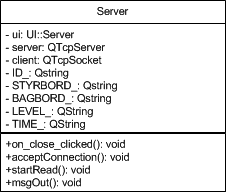
\includegraphics[width=0.4\textwidth]{billeder/serverKlassediagram}
	\caption{Klassedigram for databasens severer}
	\label{fig:serverKlassediagram}
\end{figure}

\begin{figure}[H]
	\centering
	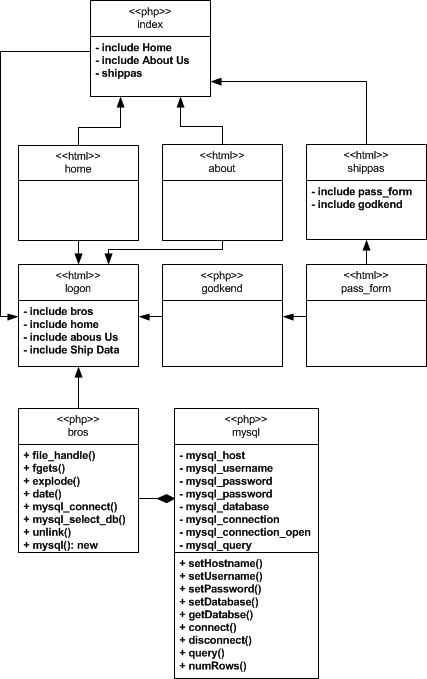
\includegraphics[width=0.5\textwidth]{billeder/web_klasse}
	\caption{Klassedigram for databasens web-side.}
	\label{fig:serverKlassediagram}
\end{figure}
\fxnote{check med kim, beskriv <<html>> og <<php>>}


\subsection{Funktionsbeskrivelser}
\subsubsection{Server}
Denne header står for at starte serveren og starte GUI for korte informationer til brugeren. Alle informationer om server start, connection og datamodtagelse vil blive udskrevet her. 

\begin{table}[H]
\begin{tabular}{l p{12.5cm}}
\multicolumn{2}{l}{\texttt{\textcolor{blue}{Void} addLogEntry( \textcolor{blue}{QString} )}} \\
\hline
Beskrivelse & Står for at udskrive beskeder fra tcp klassen til GUI \\
Parametre: & Ui::Server *ui;\\
Returværdi:& Ingen\\
\end{tabular}
\end{table}

\begin{table}[H]
\begin{tabular}{l p{12.5cm}}
\multicolumn{2}{l}{\texttt{\textcolor{blue}{Void} on\_closeServer\_clocked( )}} \\
\hline
Beskrivelse: &Denne funktion håndtere luk knappen. Ved tryk knappen vil brugeren blive bedt om at svare ja eller nej til at lukke server connectionen \\
Parametre: & Ingen\\
Returværdi: & Ingen\\
\end{tabular}
\end{table}

\begin{table}[H]
\begin{tabular}{l p{12.5cm}}
\multicolumn{2}{l}{\texttt{\textcolor{blue}{Void} on\_webDatabase\_clicked( )}} \\
\hline
Beskrivelse: & Denne funktion står for at håndtere den direkte adgang til den web baserede database. Ved tryk vil brugeren få åbnet et nyt vindue med database adgang \\
Parametre: & QWebView* m\_pWebView\\
Returværdi: & Ingen\\
\end{tabular}
\end{table}

\subsubsection{update}
Denne header står for at håndtere de struct's der benyttes til at at save data til log filen. 

\begin{table}[H]
\begin{tabular}{l p{12.5cm}}
\multicolumn{2}{l}{\texttt{\textcolor{blue}{Void} addLogEntry( \textcolor{blue}{QString} )}} \\
\hline
Beskrivelse&Står for at udskrive beskeder fra tcp klassen til GUI \\
Parametre:& Ui::Server *ui;\\
Returværdi:&\\
\end{tabular}
\end{table}


\subsubsection{tcp}
Denne header står for tcp forbindelsen. Socket oprettes og connection adgang gives. Når data bliver modtaget blvier denne gemt i den eksterne log fil ship.txt

\begin{table}[H]
\begin{tabular}{l p{12.5cm}}
\multicolumn{2}{l}{\texttt{\textcolor{blue}{Void} addLogEntry( \textcolor{blue}{QString} )}} \\
\hline
Beskrivelse: & Står for at udskrive beskeder fra tcp klassen til GUI \\
Parametre: & Ui::Server *ui;\\
Returværdi:&\\
\end{tabular}
\end{table}

\begin{table}[H]
\begin{tabular}{l p{12.5cm}}
\multicolumn{2}{l}{\texttt{\textcolor{blue}{Void} acceptConnection( \textcolor{blue}{void} )}} \\
\hline
Beskrivelse:&Står for at acceptere forbindelse fra KI og connecte.\\
Parametre:&QTcpServer server\\
				&QTcpSocket* client\\
Returværdi:&\\
\end{tabular}
\end{table}

\begin{table}[H]
\begin{tabular}{l p{12.5cm}}
\multicolumn{2}{l}{\texttt{\textcolor{blue}{Void} startRead( \textcolor{blue}{void} )}} \\
\hline
Beskrivelse:&Læser data fra socket. Data til fil og GUI\\
Parametre:&QTcpSocket* client\\
Returværdi:&\\
\end{tabular}
\end{table}

\subsubsection{savedata}
Denne header står for at handtere lagring af data modtaget fra skibet. Den lager dataerne i ship.txt

\begin{table}[H]
\begin{tabular}{l p{12.5cm}}
\multicolumn{2}{l}{\texttt{\textcolor{blue}{int} save( \textcolor{blue}{save\_data} )}} \\
\hline
Beskrivelse & Står for at udskrive beskeder fra tcp klassen til GUI \\
Parametre: & Ingen\\
Returværdi:& Ingen\\
\end{tabular}
\end{table}

\subsubsection{Wep-side}
Web-siden står for at fremvise skibs data grafisk for terminal personalet. Desuden står den for at lager data og loade data fra mySQL databasen.\\

\subsubsection{bros}

\begin{table}[H]
\begin{tabular}{l p{12.5cm}}
\multicolumn{2}{l}{\texttt{\textcolor{blue}{} file\_handle( \textcolor{blue}{} )}} \\
\hline
Beskrivelse:&Læse hvilken adresse databasen ligger på\\
Parametre:& Ingen\\
Returværdi:& Ingen\\
\end{tabular}
\end{table}

\begin{table}[H]
\begin{tabular}{l p{12.5cm}}
\multicolumn{2}{l}{\texttt{\textcolor{blue}{} fgets ( \textcolor{blue}{} )}} \\
\hline
Beskrivelse:&Læse hvilken adresse databasen ligger på\\
Parametre:& Ingen\\
Returværdi:& Ingen\\
\end{tabular}
\end{table}

\begin{table}[H]
\begin{tabular}{l p{12.5cm}}
\multicolumn{2}{l}{\texttt{\textcolor{blue}{} explode( \textcolor{blue}{} )}} \\
\hline
Beskrivelse: &Læse hvilken adresse databasen ligger på\\
Parametre: & Ingen\\
Returværdi: & Ingen\\
\end{tabular}
\end{table}

\begin{table}[H]
\begin{tabular}{l p{12.5cm}}
\multicolumn{2}{l}{\texttt{\textcolor{blue}{} date( \textcolor{blue}{} )}} \\
\hline
Beskrivelse: &Opdatere dato og tid når der gemmes til mySQL databasen\\
Parametre: & Ingen\\
Returværdi: & Ingen\\
\end{tabular}
\end{table}

\begin{table}[H]
\begin{tabular}{l p{12.5cm}}
\multicolumn{2}{l}{\texttt{\textcolor{blue}{} mysql\_connect( \textcolor{blue}{} )}} \\
\hline
Beskrivelse: &Læse hvilken adresse databasen ligger på\\
Parametre: & Ingen\\
Returværdi: & Ingen\\
\end{tabular}
\end{table}

\begin{table}[H]
\begin{tabular}{l p{12.5cm}}
\multicolumn{2}{l}{\texttt{\textcolor{blue}{} mysql\_select\_db( \textcolor{blue}{} )}} \\
\hline
Beskrivelse: & Læse hvilken adresse databasen ligger på\\
Parametre: & Ingen\\
Returværdi: & Ingen\\
\end{tabular}
\end{table}

\begin{table}[H]
\begin{tabular}{l p{12.5cm}}
\multicolumn{2}{l}{\texttt{\textcolor{blue}{} unlink( \textcolor{blue}{} )}} \\
\hline
Beskrivelse: & Læse hvilken adresse databasen ligger på\\
Parametre: & Ingen\\
Returværdi: & Ingen\\
\end{tabular}
\end{table}

\begin{table}[H]
\begin{tabular}{l p{12.5cm}}
\multicolumn{2}{l}{\texttt{\textcolor{blue}{new} mysql( \textcolor{blue}{} )}} \\
\hline
Beskrivelse: & Læse hvilken adresse databasen ligger på\\
Parametre: & Ingen\\
Returværdi: & Ingen\\
\end{tabular}
\end{table}

\subsubsection{mysql}
\begin{table}[H]
\begin{tabular}{l p{12.5cm}}
\multicolumn{2}{l}{\texttt{\textcolor{blue}{} setHostName( \textcolor{blue}{} )}} \\
\hline
Beskrivelse: & Læse hvilken adresse databasen ligger på\\
Parametre: & Ingen\\
Returværdi: & Ingen\\
\end{tabular}
\end{table}

\begin{table}[H]
\begin{tabular}{l p{12.5cm}}
\multicolumn{2}{l}{\texttt{\textcolor{blue}{} setUserName( \textcolor{blue}{} )}} \\
\hline
Beskrivelse: & Skriver brugernavn til databasen\\
Parametre: & Ingen\\
Returværdi: & Ingen\\
\end{tabular}
\end{table}

\begin{table}[H]
\begin{tabular}{l p{12.5cm}}
\multicolumn{2}{l}{\texttt{\textcolor{blue}{} setPassword( \textcolor{blue}{} )}} \\
\hline
Beskrivelse:&Skriver password til databasen\\
Parametre: & Ingen\\
Returværdi: & Ingen\\
\end{tabular}
\end{table}

\begin{table}[H]
\begin{tabular}{l p{12.5cm}}
\multicolumn{2}{l}{\texttt{\textcolor{blue}{} setDatabase( \textcolor{blue}{} )}} \\
\hline
Beskrivelse: & Fortæller mySQL hvilken database der skal benyttes\\
Parametre: & Ingen\\
Returværdi: & Ingen\\
\end{tabular}
\end{table}

\begin{table}[H]
\begin{tabular}{l p{12.5cm}}
\multicolumn{2}{l}{\texttt{\textcolor{blue}{} getDatabase( \textcolor{blue}{} )}} \\
\hline
Beskrivelse: & Tager fat i databasen\\
Parametre: & Ingen\\
Returværdi: & Ingen\\
\end{tabular}
\end{table}

\begin{table}[H]
\begin{tabular}{l p{12.5cm}}
\multicolumn{2}{l}{\texttt{\textcolor{blue}{} connect( \textcolor{blue}{} )}} \\
\hline
Beskrivelse: & Står for at samle localhost, username, password, database og connecte til databasen\\
Parametre: & Ingen\\
Returværdi: & Ingen\\
\end{tabular}
\end{table}

\begin{table}[H]
\begin{tabular}{l p{12.5cm}}
\multicolumn{2}{l}{\texttt{\textcolor{blue}{} disconnect( \textcolor{blue}{} )}} \\
\hline
Beskrivelse: & Lukker database forbindelsen\\
Parametre: & Ingen\\
Returværdi: & Ingen\\
\end{tabular}
\end{table}

\begin{table}[H]
\begin{tabular}{l p{12.5cm}}
\multicolumn{2}{l}{\texttt{\textcolor{blue}{} query( \textcolor{blue}{} )}} \\
\hline
Beskrivelse: & Opretter database kø og skriver data til skærm\\
Parametre: & Ingen\\
Returværdi: & Ingen\\
\end{tabular}
\end{table}

\begin{table}[H]
\begin{tabular}{l p{12.5cm}}
\multicolumn{2}{l}{\texttt{\textcolor{blue}{} numRows( \textcolor{blue}{} )}} \\
\hline
Beskrivelse: & Checker hvor mange rækker der findes i databasen bruges desuden til at udskrive om databasen er tom.\\
Parametre: & Ingen\\
Returværdi: & Ingen\\
\end{tabular}
\end{table}

\subsection{Tilpasning}
Der er mulighed for at opsætte server delen sådan at denne lagre direkte i mySQL databsen hvis man har et ønske om at mindske ansvaret for websiden. for at gøre dette kan man i tcp klassens funktion startRead(void) erstate funktionskaldet til klassen savedata() med funktionen save(tmp) og i stedet benytte klassen SQL med funktionskaldet saveSQL(tmp). funktionen saveSQL(tmp) har save(tmp) som i tilfælde af at der opstår fejl med at gemme data til databasen vil sikre at data bliver lagret i en backup fil som så kan håndteres af websiden.

\subsection{Apache}
Apache HTTP Server er en webserver fra Apache Software Foundation. Apache er en ofte benytte webserver og er en open source-serverprogram. Serveren installeres på en computer og kan herefter benytte ved at benytte den lokale ip adresse 127.0.0.1 eller localhost. Om computeren med Apache serveren er placeret i et større netværk og skal benyttes fra andre computere kan denne tilgås fra disse ved at indtaste computerens oprindelige ip adresse på netværket. Dette giver også mulighed for at benytte serveren fra internettet ved at koble den op via DNS. Om dette gøres skal man specielt være opmærksom på at lukke port numrerne 20 og 21 da disse ofte er portene som bliver hacket desuden bør man ligge password på serveren for udefra kommende. I BROS er Apache serveren placeret i internt netværk og derfor er det ikke nødvendigt at lukke portene eller benytte sig af password tilladelse for at arbejde til serveren.
Generalt står apache serverene for ca 60\% af alle webserere i verden.
fxnote{kilde: IKN bog og wikipedia} 

\subsection{mySQL}
MySQL er en flertrådet SQL-databaseserver som understøtter mange samtidige brugere. SQL(Structured Query Language) er det mest populere databasesprog i dag. MySQLer et klient/server-program der består af en server (mysqld) og mange forskellige klientprogrammer.\\
MySQL er bygget op omkring forskellige databaser på en server, ofte har hver enkelt bruger en speciel adgang til en databse med en overordnet root bruger der har adgang til alle databaser.\\
MySQL er en relationel dabase hvori man kan oprette flere taballer til at håndtere flere ting. I BROS Databasen benyttes der en database med navnet bros. I denne database kan der oprettes taballer til de skibe der skal kunne gemems data for. C++ og php er istand til at se på om en tabel er oprettet, hvis den ikke er det kan sprogene selv oprette disse(dette er ikke indkodet da vi kun arbejder emd et skib). \\
Til at tilgå mySQL kan man benytte sig af terminalen \footnote{beskrevet i apendix} eller grafisk brugergrænseflade som f.eks. phpMyAdmin (benyttet under udviklingen).
MySQL kan benytte flere forskellige datatyper som vil blive beskrevet i apandix for mySQL. 






